%==============================================================================
%  MEMORIA DE CÁLCULO — Electrónica de la plataforma QUBE (ESP32)
%  Documento autocontenido: compila con  pdflatex memoria_calculo_electronica.tex
%  (dos pasadas para las referencias cruzadas).
%
%  Para incrustarlo en la tesis: borrar el preámbulo y el \begin/\end{document},
%  dejar sólo desde "\section{...}" en adelante, e incluirlo con \input{}.
%==============================================================================
\documentclass[11pt,letterpaper]{article}
\usepackage[utf8]{inputenc}
\usepackage[T1]{fontenc}
\usepackage[spanish,es-nodecimaldot]{babel}
\usepackage{amsmath,amssymb}
\usepackage{booktabs}
\usepackage{graphicx}
\usepackage{float}
\usepackage{siunitx}
\usepackage[margin=2.5cm]{geometry}
\usepackage[hidelinks]{hyperref}
\usepackage{enumitem}

\sisetup{
  output-decimal-marker = {,},
  separate-uncertainty  = true,
  per-mode              = symbol,
}
\graphicspath{{.}{imagenes/}}

\title{\textbf{Memoria de cálculo de la electrónica de acondicionamiento y potencia}\\[2pt]
       \large Plataforma de péndulo invertido QUBE — ESP32}
\author{Antonio José Badilla Torrealba}
\date{Universidad de Santiago de Chile — 2026}

\begin{document}
\maketitle

\begin{abstract}
\noindent
Este documento justifica, paso a paso, la selección de cada resistencia y
condensador de la placa de la plataforma QUBE. Para cada componente se enuncia
su \emph{función}, la \emph{ecuación} que gobierna su dimensionamiento, la
\emph{sustitución numérica} con los valores del diseño y el \emph{resultado}, y
se discute su \emph{significancia} dentro del sistema. Los bloques tratados son:
protección (fusible), sensado de corriente (INA219), regulación de \SI{5}{V}
(LM2596), acondicionamiento de encoders (pull-ups, Schmitt trigger CD40106BE,
filtro RC) y la red de desacople (condensadores de bypass y \emph{bulk}), más la
topología de tierra en estrella.
\end{abstract}

\tableofcontents
\bigskip

%------------------------------------------------------------------------------
\section{Topología general y árbol de alimentación}
%------------------------------------------------------------------------------
El sistema se organiza en tres dominios de tensión que parten de una única
fuente de \SI{15}{V}\,DC y comparten una tierra común en configuración de
estrella (Figura~\ref{fig:wiring}):

\begin{enumerate}[nosep]
  \item \textbf{Potencia de motor (\SI{15}{V}):} Fuente $\to$ fusible \SI{1.5}{A}
        $\to$ resistencia \emph{shunt} del INA219 $\to$ terminal \texttt{VS} del
        driver BTS7960 $\to$ motor DC.
  \item \textbf{Lógica (\SI{5}{V}):} regulador reductor LM2596 (\SI{15}{}$\to$\SI{5}{V})
        que alimenta el ESP32 (\texttt{VIN}), la lógica del BTS7960 (\texttt{VCC})
        y los encoders.
  \item \textbf{Lógica (\SI{3.3}{V}):} regulador interno del ESP32 (pin \texttt{3V3})
        que alimenta el \texttt{Vcc} de los CD40106BE y los pull-ups de los
        encoders.
\end{enumerate}

\begin{figure}[H]
  \centering
  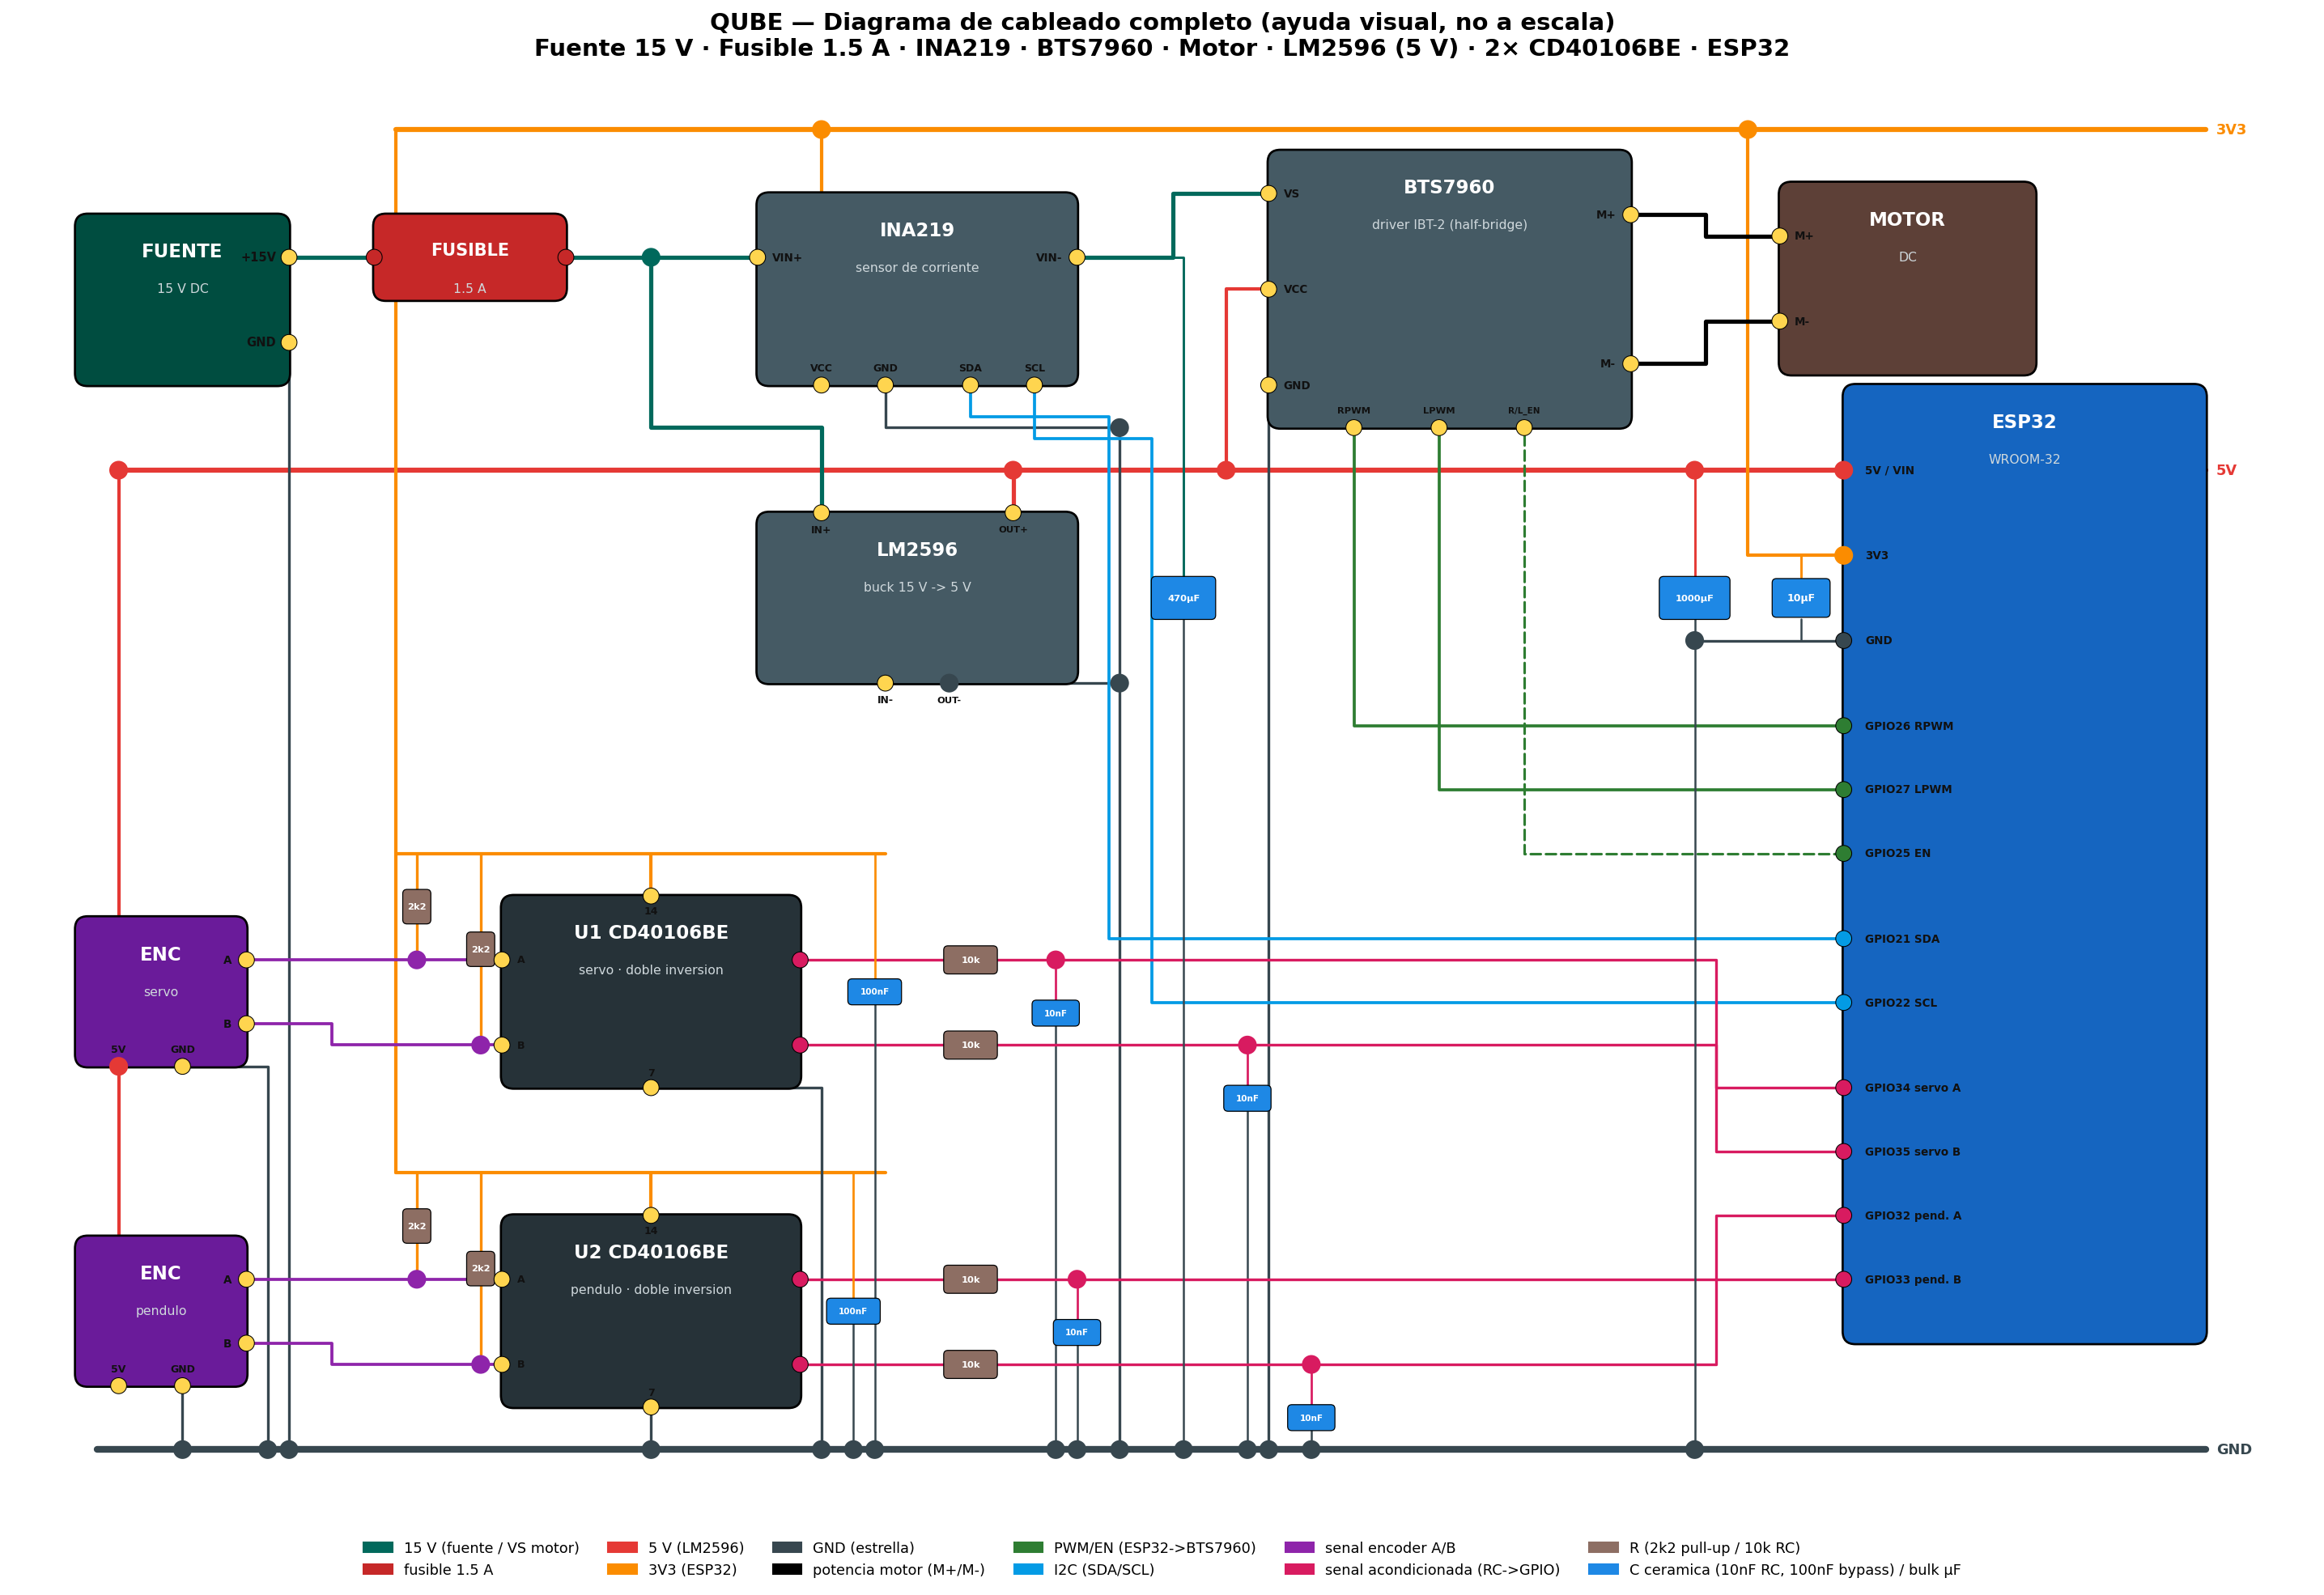
\includegraphics[width=\linewidth]{system_wiring.png}
  \caption{Diagrama de cableado completo del sistema (ayuda visual, no a escala).}
  \label{fig:wiring}
\end{figure}

\paragraph{Parámetros de diseño asumidos.}
Los cálculos usan los valores de la Tabla~\ref{tab:param}, tomados del BOM y de
las hojas de datos de los componentes.

\begin{table}[H]
  \centering
  \caption{Parámetros de diseño de referencia.}
  \label{tab:param}
  \begin{tabular}{lll}
    \toprule
    Símbolo & Descripción & Valor \\
    \midrule
    $V_\text{s}$        & Tensión de fuente (potencia de motor) & \SI{15}{V} \\
    $P_\text{mot}$      & Potencia nominal del motor            & \SI{25}{W} \\
    $V_\text{cc}$       & Rail lógico del CD40106BE / pull-ups  & \SI{3.3}{V} \\
    $f_\text{PWM}$      & Frecuencia de conmutación del BTS7960 & \SI{20}{kHz} \\
    $N$                 & Resolución del encoder (mín.)         & \SI{200}{CPR} \\
    $n_\text{max}$      & Velocidad máx. del eje (motor)        & \SI{300}{rpm} \\
    $R_\text{sh}$       & Shunt interno del INA219              & \SI{0.1}{\ohm} \\
    $V_\text{ref}$      & Referencia de realimentación LM2596   & \SI{1.23}{V} \\
    \bottomrule
  \end{tabular}
\end{table}

%------------------------------------------------------------------------------
\section{Protección: fusible de \texorpdfstring{\SI{1.5}{A}}{1.5 A}}
%------------------------------------------------------------------------------
\paragraph{Función.} Interrumpir la alimentación de potencia ante un cortocircuito
en el motor o el driver, o ante una corriente sostenida anómala (rotor bloqueado).

\paragraph{Corriente nominal del motor.} En el peor caso de potencia nominal,
\begin{equation}
  I_\text{mot,nom} = \frac{P_\text{mot}}{V_\text{s}}
  = \frac{\SI{25}{W}}{\SI{15}{V}} = \SI{1.67}{A}.
  \label{eq:imot}
\end{equation}

\paragraph{Corriente real de operación.} Durante el equilibrado del péndulo el par
requerido es una fracción del nominal, de modo que la corriente eficaz típica es
$I_\text{rms}\ll I_\text{mot,nom}$ (del orden de algunas centenas de \si{mA}). El
pico se da en el \emph{swing-up}.

\paragraph{Selección.} Se elige un fusible \emph{lento} (\emph{time-lag}, T) de
\SI{1.5}{A}. El criterio es:
\begin{equation}
  I_\text{rms,operación} \;<\; I_\text{fusible} \;<\; I_\text{daño del cableado},
  \qquad
  \SI{0.5}{A} < \SI{1.5}{A} < I_\text{daño}.
\end{equation}
El carácter lento aprovecha la característica $I^2t$ del fusible: tolera los picos
breves del \emph{swing-up} sin fundirse, pero abre ante una corriente sostenida
(p.\,ej.\ rotor bloqueado, donde $I_\text{stall}=V_\text{s}/R_\text{arm}$ alcanza
varios amperios) o un cortocircuito.

\paragraph{Significancia.} El fusible es la última línea de defensa contra un fallo
que, de otro modo, descargaría la fuente (o la batería LiPo) a través del bobinado
o del puente~H. \emph{Nota de diseño:} si se requiere operación sostenida a
potencia nominal (Ec.~\ref{eq:imot} $=\SI{1.67}{A}>\SI{1.5}{A}$), conviene subir el
fusible a \SI{2}{A}.

%------------------------------------------------------------------------------
\section{Sensado de corriente: INA219 y su \emph{shunt}}
%------------------------------------------------------------------------------
El INA219 mide la corriente del motor por la caída en una resistencia \emph{shunt}
de precisión $R_\text{sh}=\SI{0.1}{\ohm}$ colocada en el lado alto (entre
\texttt{VIN+} y \texttt{VIN$-$}, antes del BTS7960).

\paragraph{Caída de tensión en el shunt.}
\begin{equation}
  V_\text{sh} = I\,R_\text{sh}
  = \SI{1.67}{A}\times\SI{0.1}{\ohm} = \SI{167}{mV}.
\end{equation}
El amplificador del INA219 admite hasta \SI{\pm320}{mV} (ganancia PGA $/8$), por lo
que el rango de medida es
\begin{equation}
  I_\text{max} = \frac{\SI{320}{mV}}{R_\text{sh}}
  = \frac{\SI{0.320}{V}}{\SI{0.1}{\ohm}} = \SI{3.2}{A},
\end{equation}
coherente con el rango $\pm\SI{3.2}{A}$ del módulo y con holgura sobre
$I_\text{mot,nom}$.

\paragraph{Potencia disipada en el shunt.}
\begin{equation}
  P_\text{sh} = I^2 R_\text{sh}
  = (\SI{1.67}{A})^2\times\SI{0.1}{\ohm} = \SI{0.28}{W}.
\end{equation}
Exige un shunt de $\ge\SI{0.5}{W}$ (los módulos traen típicamente \SI{2}{W}).

\paragraph{Calibración (resolución).} Fijando una corriente máxima esperada de
\SI{3.2}{A} sobre los 15 bits del registro:
\begin{align}
  \text{Current\_LSB} &= \frac{I_\text{max}}{2^{15}}
     = \frac{\SI{3.2}{A}}{32768} \approx \SI{97.7}{\micro A}
     \;\to\; \SI{100}{\micro A}, \\[2pt]
  \text{CAL} &= \operatorname{trunc}\!\left(
     \frac{0{,}04096}{\text{Current\_LSB}\cdot R_\text{sh}}\right)
     = \frac{0{,}04096}{\SI{100e-6}{}\times\SI{0.1}{}} = 4096.
\end{align}

\paragraph{Significancia.} Con \SI{100}{\micro A} de resolución, el INA219 permite
estimar par y detectar sobrecorrientes por software (protección complementaria al
fusible), a costa de una caída despreciable (\SI{167}{mV} sobre \SI{15}{V}, un
\SI{1.1}{\percent}).

%------------------------------------------------------------------------------
\section{Regulación de \texorpdfstring{\SI{5}{V}}{5 V}: convertidor LM2596}
%------------------------------------------------------------------------------
\paragraph{Función.} Convertir los \SI{15}{V} de potencia a un rail de \SI{5}{V}
para la lógica (ESP32, lógica del BTS7960, encoders).

\paragraph{Tensión de salida (divisor de realimentación).} En la versión ajustable,
\begin{equation}
  V_\text{out} = V_\text{ref}\left(1+\frac{R_2}{R_1}\right)
  \;\Rightarrow\;
  \frac{R_2}{R_1} = \frac{V_\text{out}}{V_\text{ref}}-1
  = \frac{\SI{5}{V}}{\SI{1.23}{V}}-1 = 3{,}07.
\end{equation}
Con $R_1=\SI{1}{k\ohm}$ resulta $R_2\approx\SI{3.07}{k\ohm}$ (ajustada por el
potenciómetro del módulo).

\paragraph{Ciclo de trabajo (ideal).}
\begin{equation}
  D = \frac{V_\text{out}}{V_\text{s}} = \frac{\SI{5}{V}}{\SI{15}{V}} = 0{,}33.
\end{equation}

\paragraph{Presupuesto de corriente del rail de \SI{5}{V}.}
\begin{table}[H]
  \centering
  \caption{Cargas del rail de \SI{5}{V}.}
  \label{tab:carga5v}
  \begin{tabular}{lll}
    \toprule
    Carga & Típica & Pico \\
    \midrule
    ESP32 (WiFi por ráfagas) & \SI{250}{mA} & \SI{500}{mA} \\
    Lógica BTS7960           & \SI{10}{mA}  & \SI{10}{mA} \\
    2 $\times$ encoder       & \SI{40}{mA}  & \SI{40}{mA} \\
    \midrule
    \textbf{Total}           & $\approx\SI{0.30}{A}$ & $\approx\SI{0.55}{A}$ \\
    \bottomrule
  \end{tabular}
\end{table}
Muy por debajo de los \SI{3}{A} del LM2596. La corriente de entrada (rendimiento
$\eta\approx0{,}85$) es
\begin{equation}
  I_\text{in} = \frac{P_\text{out}}{\eta\,V_\text{s}}
  = \frac{V_\text{out}\,I_\text{out}}{\eta\,V_\text{s}}
  = \frac{\SI{5}{V}\times\SI{0.30}{A}}{0{,}85\times\SI{15}{V}}
  = \SI{0.12}{A}.
\end{equation}

\paragraph{Significancia.} Aislar la lógica del rail ruidoso de \SI{15}{V} evita
que los transitorios del motor lleguen al ESP32; el amplio margen de corriente
garantiza que el regulador no entre en limitación durante las ráfagas de WiFi.

%------------------------------------------------------------------------------
\section{Pull-ups de los encoders: \texorpdfstring{\SI{2.2}{k\ohm}}{2.2 kOhm} a \texorpdfstring{\SI{3.3}{V}}{3.3 V}}
%------------------------------------------------------------------------------
Los encoders son de salida \textbf{open-drain (NPN)}: en estado bajo el transistor
conduce y fija \SI{0}{V}; en estado alto queda en alta impedancia y el nivel lo
impone el pull-up. Por eso el pull-up va a \SI{3.3}{V} (no a \SI{5}{V}).

\paragraph{Corriente de \emph{sink} en estado bajo.}
\begin{equation}
  I_\text{sink} = \frac{V_\text{cc}}{R_\text{pu}}
  = \frac{\SI{3.3}{V}}{\SI{2.2}{k\ohm}} = \SI{1.5}{mA}.
\end{equation}
El transistor open-drain del encoder (capaz de sumidero $\ge\SI{20}{mA}$) la maneja
con holgura. La potencia en la resistencia en ese estado es
$P=V_\text{cc}^2/R_\text{pu}=\SI{3.3}{V}^2/\SI{2.2}{k\ohm}=\SI{5.0}{mW}$.

\paragraph{Tiempo de subida del flanco.} El pull-up carga la capacidad parásita de
línea $C_\text{p}\approx\SI{30}{pF}$ (entrada + cableado):
\begin{align}
  \tau_\text{pu} &= R_\text{pu}\,C_\text{p}
     = \SI{2.2}{k\ohm}\times\SI{30}{pF} = \SI{66}{ns}, \\
  t_r\,\text{(10--90\,\%)} &\approx 2{,}2\,\tau_\text{pu} = \SI{145}{ns}.
\end{align}
Frente al espaciado entre flancos del encoder a máxima velocidad (medio periodo,
Sec.~\ref{sec:rc}, $\approx\SI{500}{\micro s}$), \SI{145}{ns} es despreciable.

\paragraph{Por qué \SI{3.3}{V} y no \SI{5}{V} (corriente de \emph{clamp}).}
Si el pull-up tirara a \SI{5}{V} contra una entrada alimentada a \SI{3.3}{V}, el
diodo de sujeción de entrada conduciría de forma continua cuando la línea reposa en
alto:
\begin{equation}
  I_\text{clamp} = \frac{V_5 - V_\text{cc} - V_\text{diodo}}{R_\text{pu}}
  = \frac{\SI{5}{V}-\SI{3.3}{V}-\SI{0.7}{V}}{\SI{2.2}{k\ohm}}
  = \SI{0.45}{mA}.
\end{equation}
Tirar a \SI{3.3}{V} anula esta corriente ($I_\text{clamp}=0$), evitando consumo
parásito y estrés del pin cuando el eje queda detenido en un tope.

\paragraph{Compromiso \SI{2.2}{}\,vs\,\SI{4.7}{k\ohm}.} \SI{2.2}{k\ohm} da flancos
más rápidos y una línea más ``rígida'' (mayor $I_\text{sink}$, \SI{1.5}{mA});
\SI{4.7}{k\ohm} reduce el consumo ($I_\text{sink}=\SI{0.70}{mA}$) a costa de un
$t_r$ mayor (\SI{310}{ns}). Ambos son válidos; se prefiere \SI{2.2}{k\ohm} por la
inmunidad al ruido.

%------------------------------------------------------------------------------
\section{Schmitt trigger CD40106BE (doble inversión)}
%------------------------------------------------------------------------------
\paragraph{Función.} Limpiar la señal del encoder eliminando rebotes y \emph{glitches}
mediante histéresis. Se usan \textbf{dos inversores por canal} (doble inversión)
para conservar la polaridad; con 4 canales se requieren 8 inversores, que no caben
en un CD40106BE (6 inversores), de ahí los \textbf{dos chips} (U1 servo, U2 péndulo).

\paragraph{Histéresis.} Con $V_\text{cc}=\SI{3.3}{V}$, los umbrales típicos son
$V_{T+}\approx\SI{2.3}{V}$ y $V_{T-}\approx\SI{1.0}{V}$, de donde la banda muerta es
\begin{equation}
  \Delta V_T = V_{T+}-V_{T-} \approx \SI{2.3}{V}-\SI{1.0}{V} = \SI{1.3}{V}.
\end{equation}
Cualquier ruido de amplitud menor a \SI{1.3}{V} superpuesto a la señal \emph{no}
provoca conmutación espuria: esta es la clave del rechazo a rebotes mecánicos y al
acoplo del PWM.

\paragraph{Significancia.} La histéresis convierte una transición lenta o ruidosa
en un flanco digital limpio ($t_\text{prop}\approx\SI{80}{}$--\SI{150}{ns}), lo que
elimina las cuentas espurias del contador de cuadratura.

%------------------------------------------------------------------------------
\section{Filtro RC anti-alias: \texorpdfstring{\SI{10}{k\ohm}}{10 kOhm} + \texorpdfstring{\SI{10}{nF}}{10 nF}}
\label{sec:rc}
%------------------------------------------------------------------------------
Tras cada salida del Schmitt se coloca un filtro paso-bajo de primer orden antes
del GPIO.

\paragraph{Constante de tiempo y frecuencia de corte.}
\begin{align}
  \tau &= R\,C = \SI{10}{k\ohm}\times\SI{10}{nF} = \SI{100}{\micro s}, \\
  f_c  &= \frac{1}{2\pi RC} = \frac{1}{2\pi\,\tau}
        = \frac{1}{2\pi\times\SI{100e-6}{s}} = \SI{1591.5}{Hz}\approx\SI{1.59}{kHz}.
\end{align}

\paragraph{Rechazo del acoplo PWM (\SI{20}{kHz}).} La magnitud del filtro es
$|H(f)|=1/\sqrt{1+(f/f_c)^2}$. En $f_\text{PWM}=\SI{20}{kHz}$:
\begin{equation}
  |H| = \frac{1}{\sqrt{1+\left(\dfrac{\SI{20}{kHz}}{\SI{1.59}{kHz}}\right)^2}}
      = \frac{1}{\sqrt{1+157{,}9}} = 0{,}079
      \;\;\Rightarrow\;\; \SI{-22}{dB}.
\end{equation}
El ruido de conmutación se atenúa un factor $\sim\!13$.

\paragraph{Efecto sobre la señal del encoder.} A la máxima frecuencia de canal,
\begin{equation}
  f_\text{enc,max} = \frac{n_\text{max}\,N}{60}
  = \frac{\SI{300}{rpm}\times\SI{200}{CPR}}{60} = \SI{1000}{Hz}.
\end{equation}
Como es una onda cuadrada leída contra un umbral, lo relevante no es la atenuación
de amplitud sino el \emph{retardo de flanco}:
\begin{equation}
  t_d \approx 0{,}69\,\tau = 0{,}69\times\SI{100}{\micro s} = \SI{69}{\micro s},
\end{equation}
un \SI{13.9}{\percent} del medio periodo (\SI{500}{\micro s}). Al aplicarse por
igual a ambos flancos, el \emph{ancho} del pulso se conserva y la cuenta de
cuadratura no se altera. El margen es amplio: exigiendo que $t_d$ sea menor al
\SI{25}{\percent} del medio periodo, el filtro tolera hasta
\begin{equation}
  f_\text{enc} < \frac{0{,}25}{2\,t_d} = \SI{1.81}{kHz}
  \;\;\Longleftrightarrow\;\; n < \SI{543}{rpm} > n_\text{max}.
\end{equation}

\paragraph{Significancia.} El par $R$--$C$ es un compromiso: $f_c=\SI{1.59}{kHz}$
queda \emph{por encima} de la señal útil del encoder (\SI{1}{kHz}) y \emph{muy por
debajo} del PWM (\SI{20}{kHz}), separando ambos. \emph{Nota:} con encoders de mayor
CPR habría que reducir $C$ (o $R$) para subir $f_c$.

%------------------------------------------------------------------------------
\section{Red de desacople: condensadores}
%------------------------------------------------------------------------------
La regla general es \textbf{un condensador \emph{bulk} (electrolítico) por rail}
para transitorios lentos, en paralelo con \textbf{un cerámico (\SI{100}{nF})} para
alta frecuencia, más \textbf{un cerámico de bypass por cada chip}.

\subsection{Bypass \texorpdfstring{\SI{100}{nF}}{100 nF} por chip (CD40106BE)}
\paragraph{Función.} Suministrar localmente la corriente de conmutación del chip y
ofrecer un camino de baja impedancia a alta frecuencia entre \texttt{Vcc} (pin 14)
y \texttt{GND} (pin 7).

\paragraph{Impedancia a alta frecuencia.} $Z_C = 1/(2\pi f C)$:
\begin{equation}
  Z_C\big|_{\SI{1}{MHz}} = \frac{1}{2\pi\,\SI{1e6}{Hz}\,\SI{100}{nF}}
  = \SI{1.6}{\ohm}, \qquad
  Z_C\big|_{\SI{10}{MHz}} = \SI{0.16}{\ohm}.
\end{equation}
Frente a los flancos rápidos del CMOS, el cerámico presenta una impedancia muy
baja, de modo que el pico de corriente lo entrega él y no viaja por la pista de
\texttt{Vcc} (que tiene inductancia).

\paragraph{¿Uno o dos condensadores?} La eficacia del bypass depende de estar
\emph{físicamente pegado} a los pines del integrado (lazo de baja inductancia). Un
único condensador compartido quedaría lejos de \emph{uno} de los dos chips; la
inductancia de la pista hasta el chip lejano degradaría su desacople a alta
frecuencia. Por eso se usa \textbf{uno por chip} (2 en total): es la práctica
canónica y su costo es despreciable.

\subsection{Filtro RC: cerámico de \texorpdfstring{\SI{10}{nF}}{10 nF} a GND}
Es el condensador del filtro de la Sec.~\ref{sec:rc} (4 unidades, uno por canal),
ya dimensionado ($\tau=\SI{100}{\micro s}$, $f_c=\SI{1.59}{kHz}$).

\subsection{\emph{Bulk} de \texorpdfstring{\SI{1000}{\micro F}}{1000 uF} en \texorpdfstring{\SI{5}{V}}{5 V} (anti-brownout)}
\paragraph{Función.} Sostener el rail de \SI{5}{V} durante un transitorio de
corriente más rápido que el lazo de control del LM2596 (ancho de banda $\sim$\si{kHz}),
evitando el \emph{brownout} del ESP32.

\paragraph{Caída de tensión ante un transitorio.} Con $\Delta V = I\,\Delta t / C$,
para una ráfaga de WiFi de $I=\SI{0.5}{A}$ durante $\Delta t=\SI{200}{\micro s}$:
\begin{equation}
  \Delta V = \frac{I\,\Delta t}{C}
  = \frac{\SI{0.5}{A}\times\SI{200e-6}{s}}{\SI{1000e-6}{F}}
  = \SI{0.10}{V}.
\end{equation}
El condensador limita la caída a \SI{0.10}{V} sobre \SI{5}{V} (\SI{2}{\percent}),
inofensiva para el regulador interno del ESP32. Invirtiendo la fórmula se obtiene
la capacidad mínima para una caída objetivo: $C \ge I\,\Delta t/\Delta V$.

\paragraph{Significancia.} Es el condensador \textbf{crítico}: resuelve el brownout
documentado durante el pico de corriente del \emph{swing-up}. Tensión nominal
$\ge\SI{10}{V}$ (2$\times$ el rail).

\subsection{\emph{Bulk} de \texorpdfstring{\SI{470}{\micro F}}{470 uF} en \texorpdfstring{\SI{15}{V}}{15 V} (VS del BTS7960)}
Absorbe los transitorios inductivos del motor en los bornes \texttt{VS}--\texttt{GND}.
Ante un escalón de corriente de motor $I=\SI{2}{A}$ durante $\Delta t=\SI{100}{\micro s}$
no suministrado por la fuente (por la inductancia de los cables):
\begin{equation}
  \Delta V = \frac{I\,\Delta t}{C}
  = \frac{\SI{2}{A}\times\SI{100e-6}{s}}{\SI{470e-6}{F}}
  = \SI{0.43}{V}.
\end{equation}
Mantiene \texttt{VS} estable y evita que la caída llegue al sensado y a los
reguladores. Tensión nominal $\ge\SI{25}{V}$.

\subsection{\emph{Bulk} de \texorpdfstring{\SI{10}{\micro F}}{10 uF} en \texorpdfstring{\SI{3.3}{V}}{3.3 V}}
Estabiliza el rail lógico compartido por el ESP32 y los CD40106BE, en paralelo con
un cerámico de \SI{100}{nF} para la respuesta de alta frecuencia. Se ubica junto al
pin \texttt{3V3} del ESP32.

%------------------------------------------------------------------------------
\section{Tierra en estrella}
%------------------------------------------------------------------------------
\paragraph{Función.} Evitar el acoplo por impedancia común: la corriente de retorno
del motor (amperios, conmutada a \SI{20}{kHz}) no debe compartir camino con las
señales de encoder ni con la referencia del INA219.

\paragraph{Cuantificación.} Si el retorno de señal compartiera una pista con
resistencia $R_\text{traza}=\SI{50}{m\ohm}$ con un retorno de motor de
$I_\text{mot}=\SI{2}{A}$, se inyectaría un ``rebote de tierra''
\begin{equation}
  \Delta V_\text{GND} = I_\text{mot}\,R_\text{traza}
  = \SI{2}{A}\times\SI{50}{m\ohm} = \SI{100}{mV}
\end{equation}
directamente sobre la referencia de las señales lógicas. La topología en estrella
—un único punto de unión de todas las tierras— elimina esa componente al no
compartir pista de retorno.

%------------------------------------------------------------------------------
\section{Resumen}
%------------------------------------------------------------------------------
\begin{table}[H]
  \centering
  \caption{Componentes pasivos, valor calculado y magnitud dominante.}
  \label{tab:resumen}
  \small
  \begin{tabular}{lll p{5.2cm}}
    \toprule
    Componente & Valor & Cant. & Resultado / significancia \\
    \midrule
    Fusible (T)          & \SI{1.5}{A}   & 1 & $I_\text{mot,nom}=\SI{1.67}{A}$; protege ante corto/rotor bloqueado \\
    Shunt INA219         & \SI{0.1}{\ohm}& 1 & $V_\text{sh}=\SI{167}{mV}$; $I_\text{max}=\SI{3.2}{A}$; LSB \SI{100}{\micro A} \\
    Pull-up encoder      & \SI{2.2}{k\ohm}& 4 & $I_\text{sink}=\SI{1.5}{mA}$; $t_r=\SI{145}{ns}$; sin clamp a 3V3 \\
    Serie RC             & \SI{10}{k\ohm} & 4 & con $C$: $f_c=\SI{1.59}{kHz}$ \\
    Cap. filtro RC       & \SI{10}{nF}    & 4 & $\tau=\SI{100}{\micro s}$; $-\SI{22}{dB}$ a \SI{20}{kHz} \\
    Cap. bypass          & \SI{100}{nF}   & 2 & $Z_C=\SI{0.16}{\ohm}$ a \SI{10}{MHz}; uno por chip \\
    Bulk \SI{3.3}{V}     & \SI{10}{\micro F}   & 1 & estabiliza rail lógico \\
    Bulk \SI{15}{V}      & \SI{470}{\micro F}  & 1 & $\Delta V=\SI{0.43}{V}$ ante \SI{2}{A}/\SI{100}{\micro s} \\
    Bulk \SI{5}{V}       & \SI{1000}{\micro F} & 1 & $\Delta V=\SI{0.10}{V}$; \textbf{anti-brownout} \\
    \bottomrule
  \end{tabular}
\end{table}

\noindent
Todos los valores se han verificado dentro de sus márgenes de operación: las
corrientes están muy por debajo de los límites de los dispositivos, y las
frecuencias de corte separan correctamente la señal útil del encoder (\SI{1}{kHz})
del ruido de conmutación (\SI{20}{kHz}).

\end{document}
